\begin{frame}
  \frametitle{Moderator element geometry (Zone I)}
    \begin{figure}[t]
                \vspace*{-0.2in}
                   \hspace*{-0.37in}
                \includegraphics[height=0.60\textwidth]{./images/zone_I_mesh.png}
                \vspace*{-0.05in}
                \caption{Molten Salt Breeder Reactor Zone I unit cell geometry from the reference \cite{robertson_conceptual_1971} (left) and SERPENT 2 (right).}
      \end{figure}
     
\end{frame}

\begin{frame}
  \frametitle{Full-core SERPENT model of \gls{MSBR}}
    \begin{figure}[t]
                \vspace*{-0.2in}
                   \hspace*{-0.39in}
                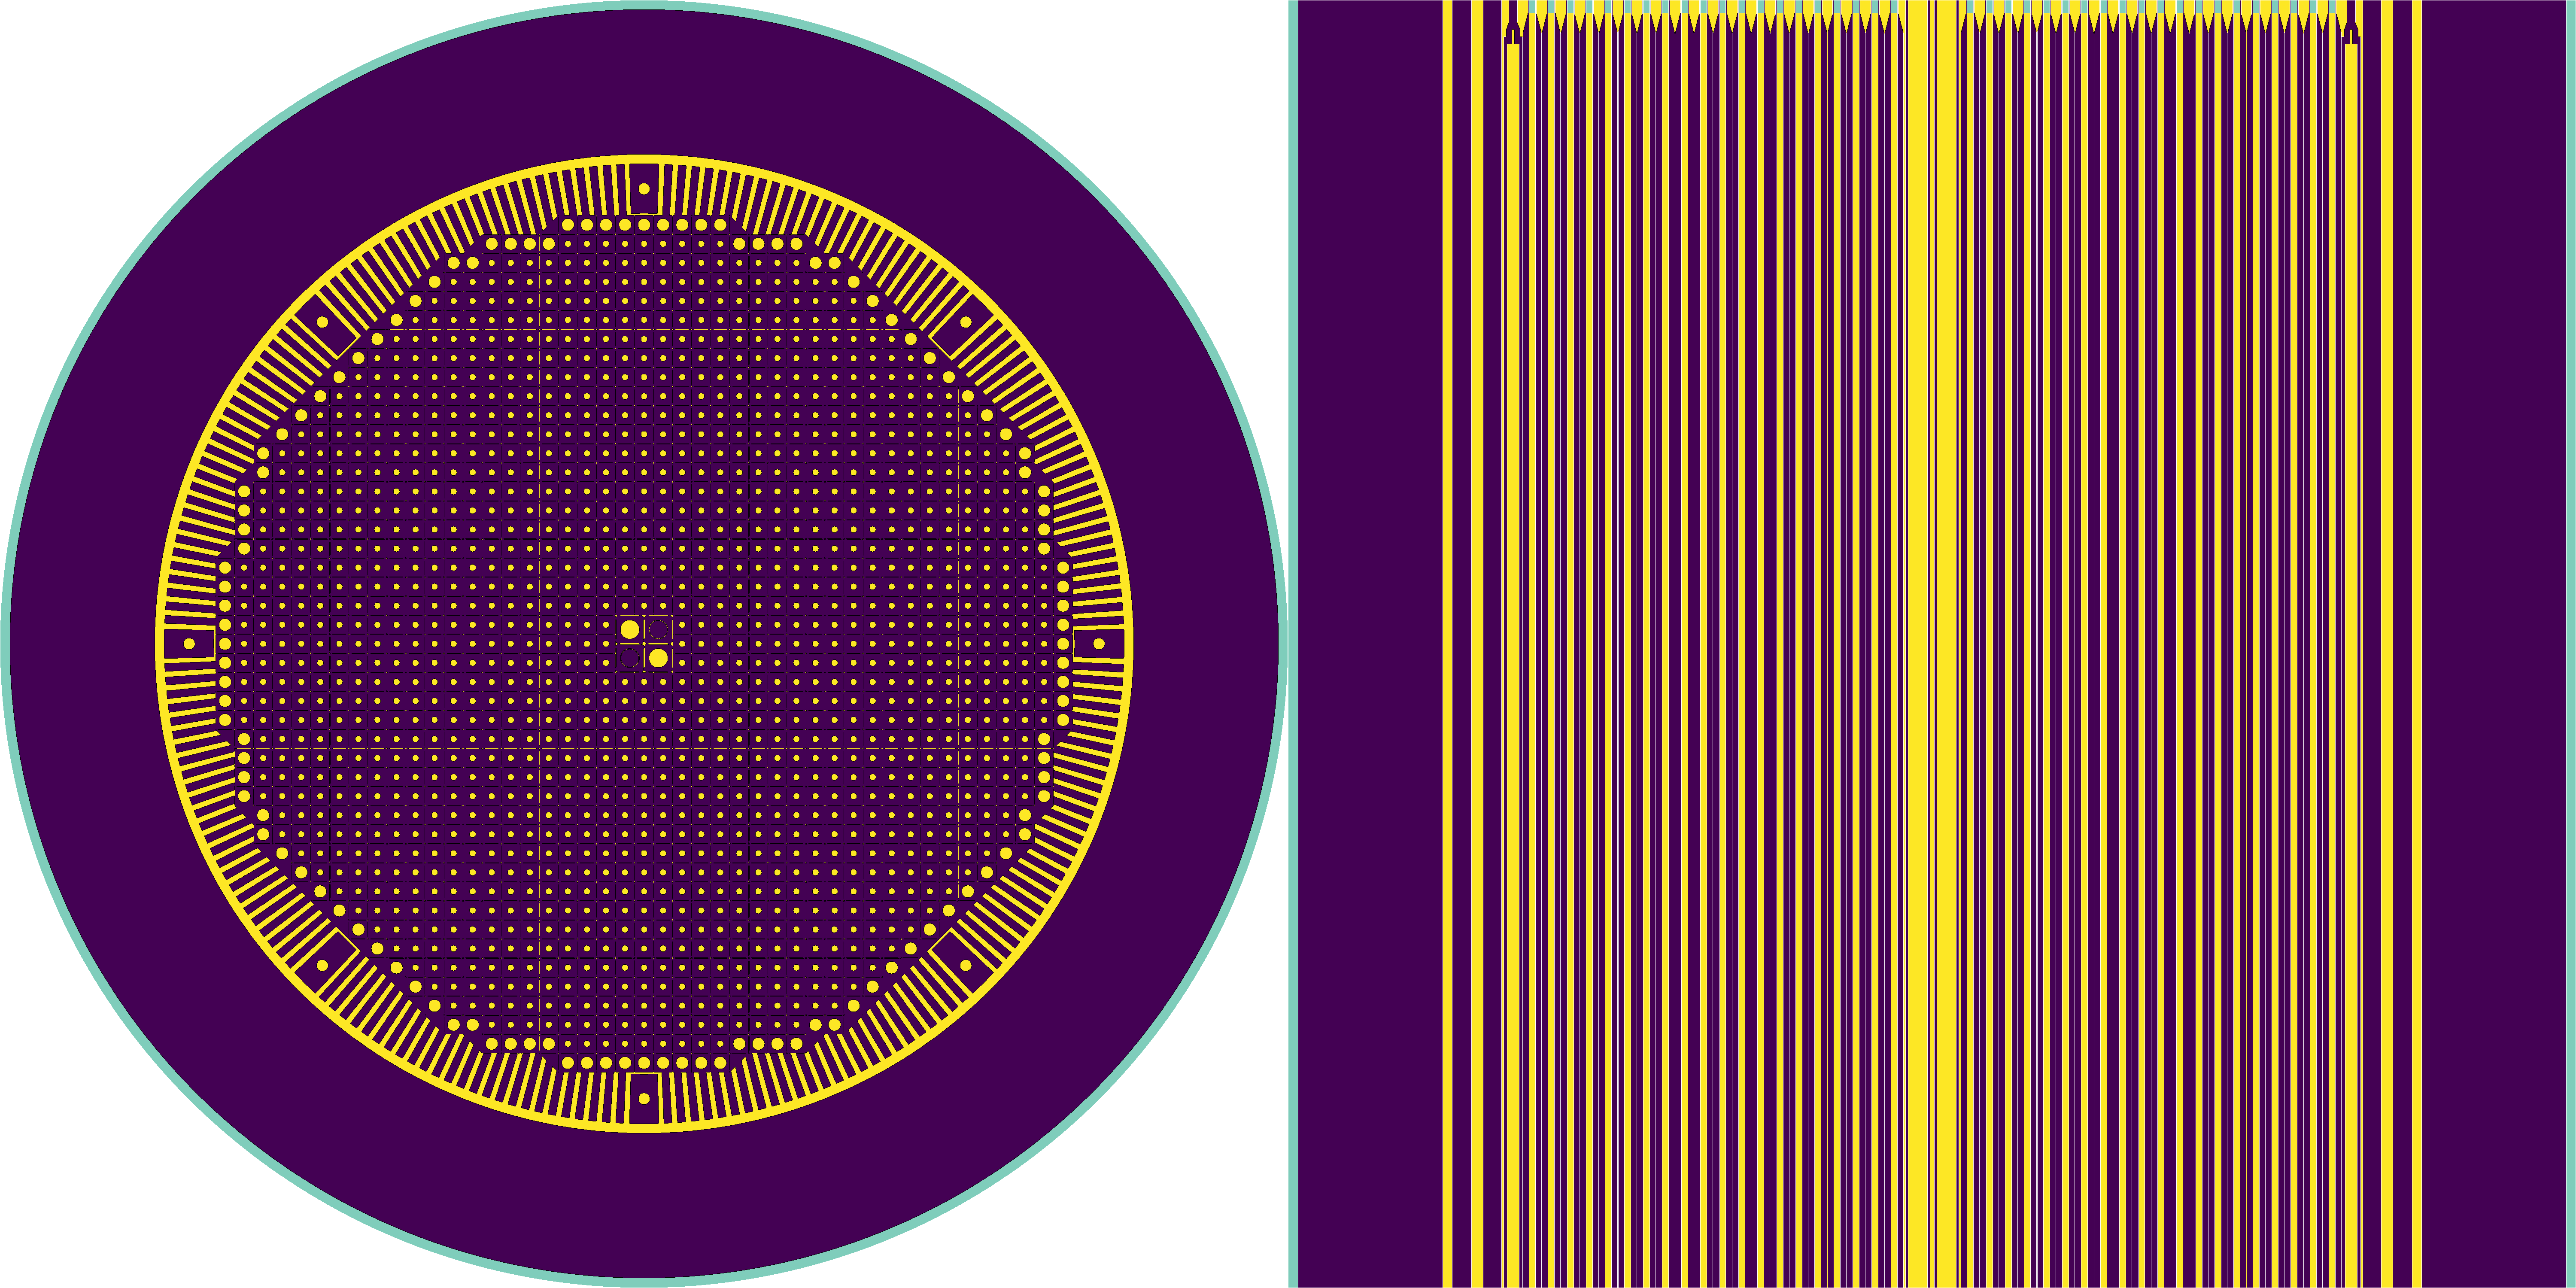
\includegraphics[height=0.6\textwidth]{./images/geometry_main_views.png}
                \caption{Plan (left) and elevation (right) view of MSBR model.}
      \end{figure}
     
\end{frame}

\begin{frame}
  \frametitle{Core Zone II}
  \begin{figure}[t]
     \vspace{-0.25in}
       \hspace*{-0.43in}
       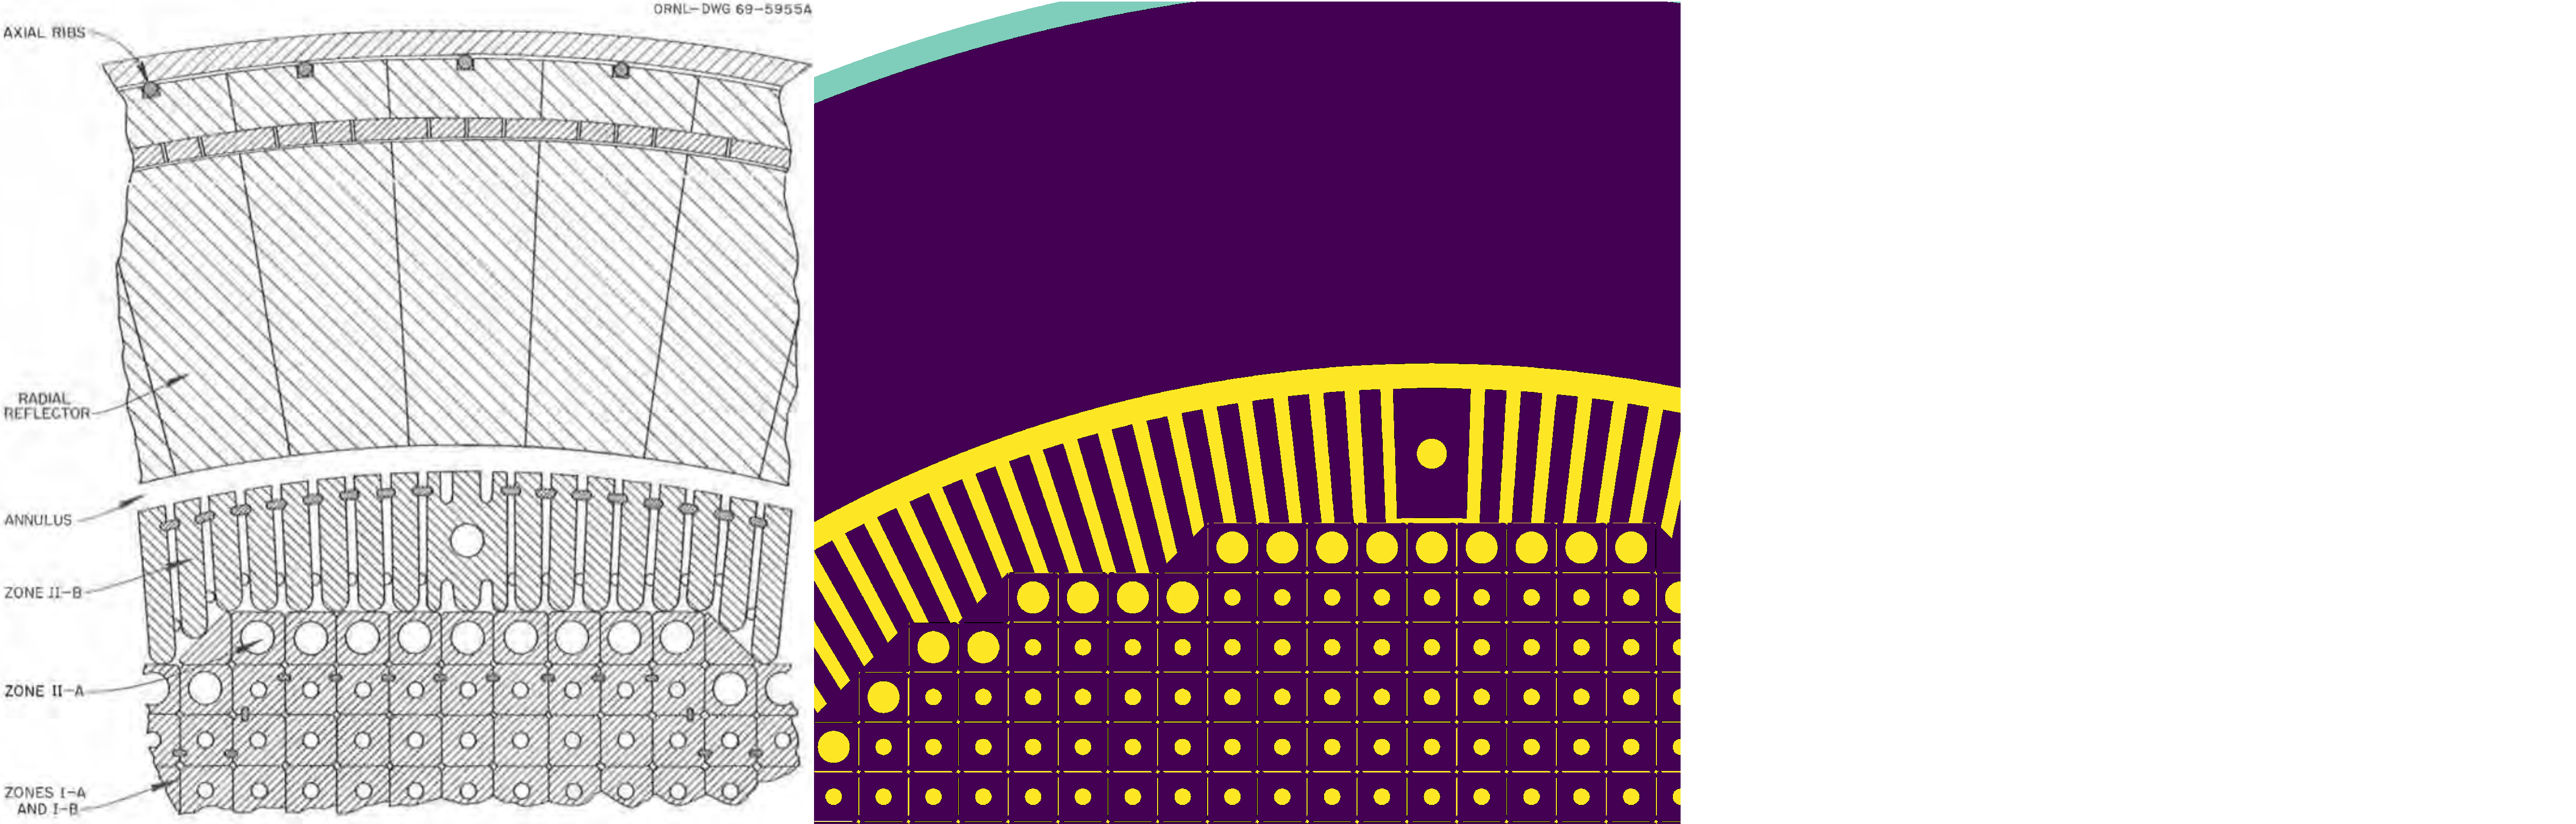
\includegraphics[height=0.77\textheight]{./images/reflector_and_elements.png}
            \caption{Detailed plan view of graphite reflector and moderator elements.}
  \end{figure}
           \vspace{-0.1in}
\end{frame}

\begin{frame}
\frametitle{Online reprocessing method}
  \begin{columns}
    \column[t]{6cm}
	\begin{figure}[t]
                \vspace*{-0.35in}
			\hspace{-0.3in}
                 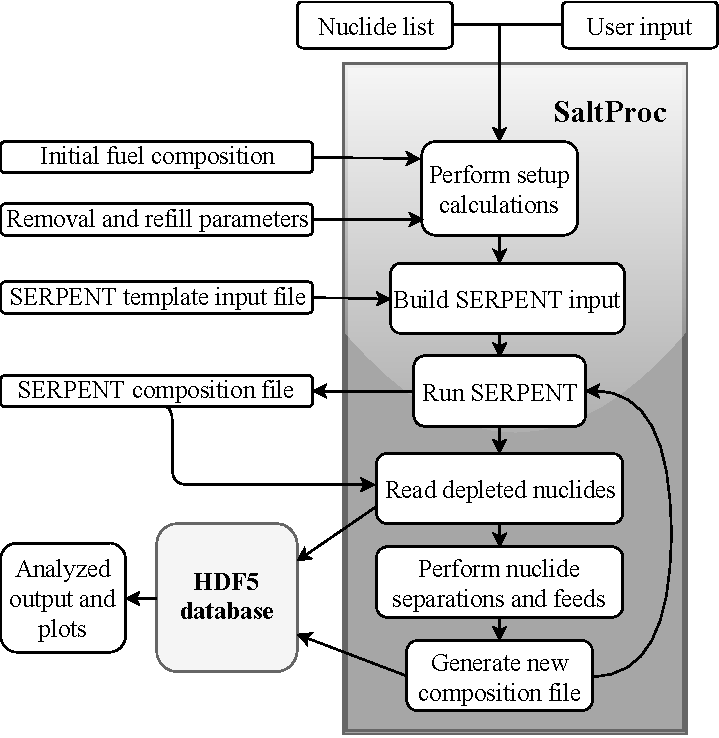
\includegraphics[height=\textwidth]{./images/saltproc_flowchart.pdf}
                \vspace*{-0.05in}
                \caption{Flow chart for the SaltProc.}
      \end{figure}

    \column[t]{6cm}
             \begin{block}{SaltProc capabilities}
               \begin{itemize}             
               \item Remove specific isotopes from the core with specific parameters (reprocessing interval, mass rate, removal efficiency)
               \item Add specific isotopes into the core
               \item Maintain constant number density of specific isotope in the core
	       \item Time-dependent material feed and removal rates
	       \item Store stream vectors in an HDF5 database for further analysis or plots
	       \item Generic geometry: an infinite medium, a unit cell, a multi-zone simplified assembly, or a full-core
               \end{itemize}
               \end{block}
  \end{columns}
\end{frame}

\begin{frame}
  \frametitle{Online reprocessing method}
     \begin{figure}[t]
                \vspace*{-0.1in}
                  % \hspace*{-0.37in}
                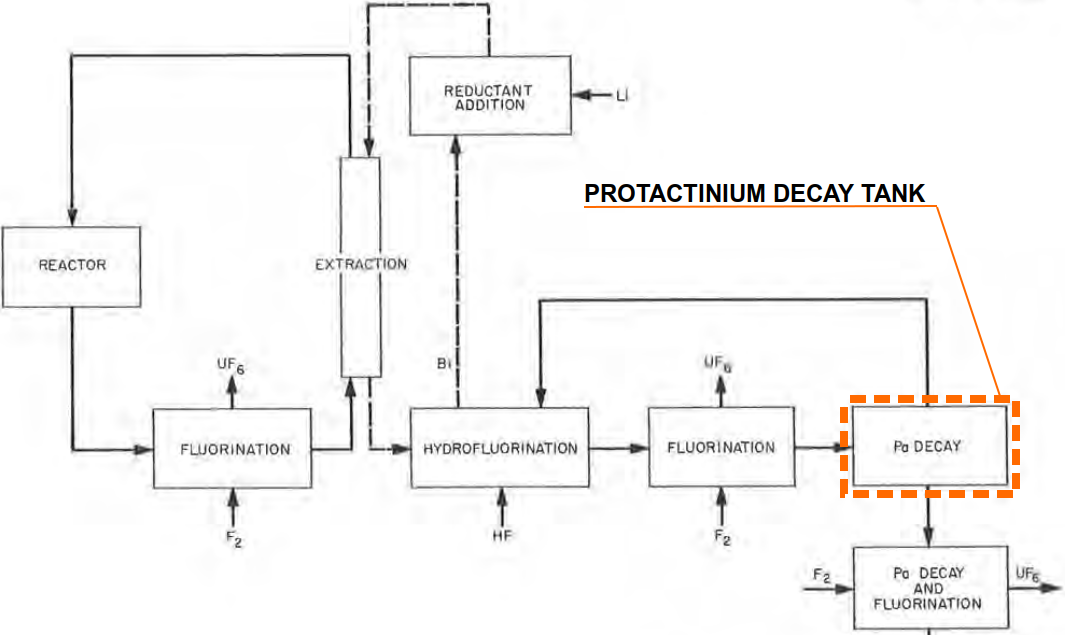
\includegraphics[height=0.45\textwidth]{./images/pa_isolation.png}
                \vspace*{-0.07in}
                \caption{Protactinium isolation with uranium removal by fluorination \cite{robertson_conceptual_1971}.}
      \end{figure}
                      \vspace*{-0.17in}
             \begin{block}{Online reprocessing approach}
               \begin{itemize}             
               \item Continuously removes all poisons, noble metals, and gases.
               \item $^{233}$Pa is continuously removed from the fuel salt into a decay tank.
               \end{itemize}
               \end{block}
               \vspace{-0.05in}
$\qquad\qquad\qquad\qquad^{232}_{90}$Th+$^1_0$n$\rightarrow^{233}_{90}$Th$\xrightarrow[\text{22.3 min}]{\beta^-}$ $^{233}_{91}$Pa$\xrightarrow[\text{26.967 d}]{\beta^-}$ $^{233}_{92}$U
\end{frame}

\begin{frame}
  \frametitle{MOOSE Framework}
  \begin{columns}
    \column[t]{6cm}
  \begin{figure}[t]
     \vspace{-0.25in}
       \hspace*{-0.25in}
       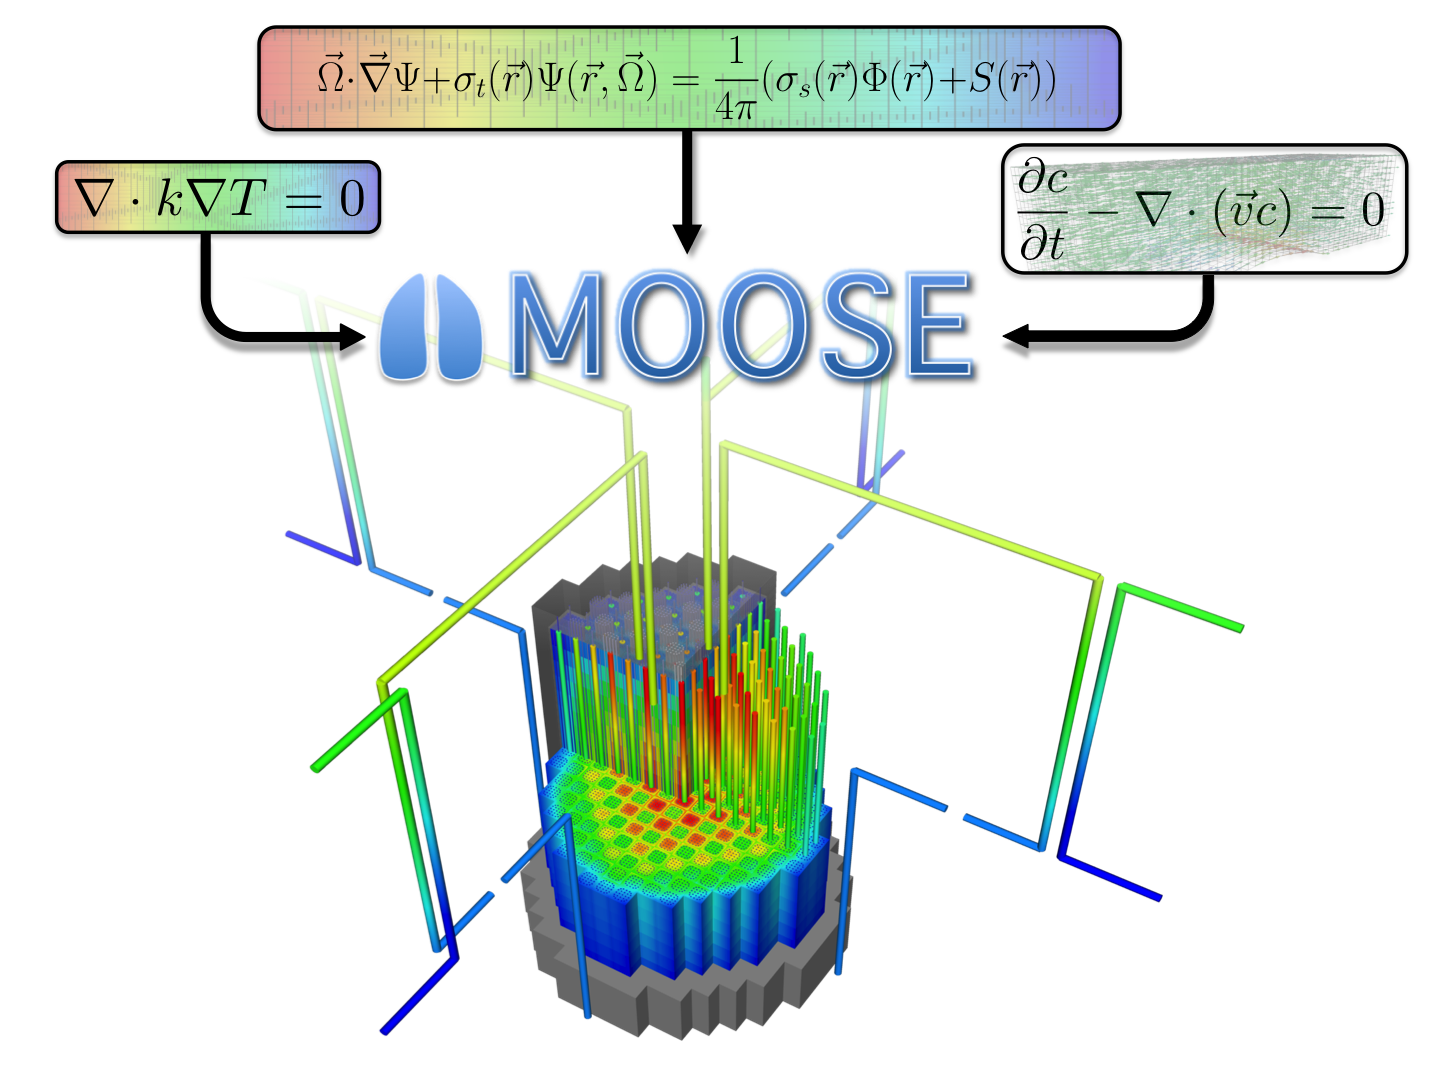
\includegraphics[height=0.65\textheight]{./images/moose.png}
            \caption{Multi-physics Object-Oriented Simulation Environment (MOOSE).}
  \end{figure}
	\column[t]{6cm}
               \begin{itemize}      
	       \item Fully-coupled, fully-implicit multiphysics solver      
               \item MOOSE interfaces with libMesh to discretize simulation volume into finite elements
               \item Residuals and Jacobians handed off to PetSc which handles solution of resulting non-linear system of algebraic equations
	       \item Automatically parallel (largest runs \textgreater 100,000 CPU cores!)
	       \item Built-in mesh adaptivity
	       \item Intuitive parallel multiscale solves
               \end{itemize}

  \end{columns}
\end{frame}

